% !TEX TS-program = xelatexmk
% !TEX encoding = UTF-8 Unicode

\documentclass[12pt]{article}
\usepackage{times}
\usepackage[margin=1in]{geometry}
\usepackage{url}
\usepackage{natbib}
\usepackage{graphicx}
\renewcommand*{\thefootnote}{\fnsymbol{footnote}}

\title{Gulliver's Travels}
\author{Jonathan Swift}
\date{An excerpt from Part III, Chapter 5\footnotemark}

\begin{document}
\maketitle
%%%%%%%%%%%%%%%%%%%%%%%%%%%%%%%%%%%%%%%%%%%%%%%%%%%%%%%%%%%%%%%%%%%%%%%%%%%%%%%%
\footnotetext{*\url{http://www.gutenberg.org/files/829/829-h/829-h.htm}}
We crossed a walk to the other part of the academy, where, as I have already said, the projectors in speculative learning resided.

\begin{figure}[!h]
\begin{center}
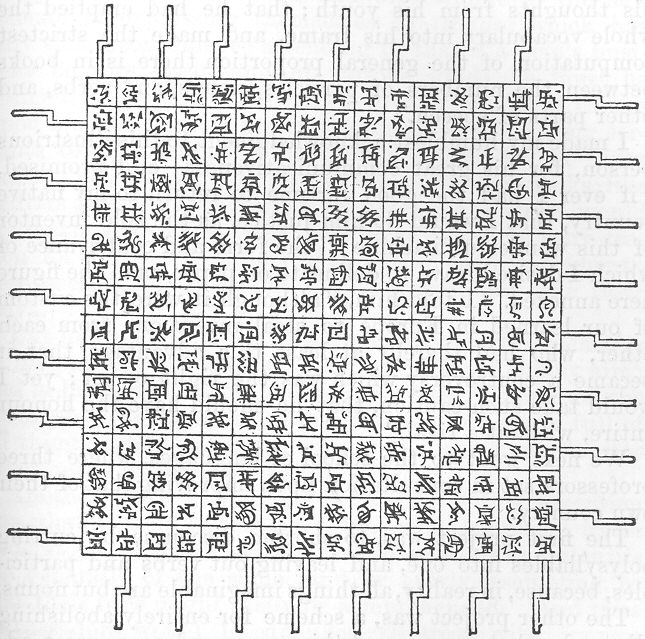
\includegraphics{1726_Gullivers_Travels_pt3_ch5_excerpt.jpg}
\end{center}
\end{figure}

The first professor I saw, was in a very large room, with forty pupils about him.  After salutation, observing me to look earnestly upon a frame, which took up the greatest part of both the length and breadth of the room, he said, “Perhaps I might wonder to see him employed in a project for improving speculative knowledge, by practical and mechanical operations.  But the world would soon be sensible of its usefulness; and he flattered himself, that a more noble, exalted thought never sprang in any other man’s head.  Every one knew how laborious the usual method is of attaining to arts and sciences; whereas, by his contrivance, the most ignorant person, at a reasonable charge, and with a little bodily labour, might write books in philosophy, poetry, politics, laws, mathematics, and theology, without the least assistance from genius or study.”  He then led me to the frame, about the sides, whereof all his pupils stood in ranks.  It was twenty feet square, placed in the middle of the room.  The superfices was composed of several bits of wood, about the bigness of a die, but some larger than others.  They were all linked together by slender wires.  These bits of wood were covered, on every square, with paper pasted on them; and on these papers were written all the words of their language, in their several moods, tenses, and declensions; but without any order.  The professor then desired me “to observe; for he was going to set his engine at work.”  The pupils, at his command, took each of them hold of an iron handle, whereof there were forty fixed round the edges of the frame; and giving them a sudden turn, the whole disposition of the words was entirely changed.  He then commanded six-and-thirty of the lads, to read the several lines softly, as they appeared upon the frame; and where they found three or four words together that might make part of a sentence, they dictated to the four remaining boys, who were scribes.  This work was repeated three or four times, and at every turn, the engine was so contrived, that the words shifted into new places, as the square bits of wood moved upside down.

Six hours a day the young students were employed in this labour; and the professor showed me several volumes in large folio, already collected, of broken sentences, which he intended to piece together, and out of those rich materials, to give the world a complete body of all arts and sciences; which, however, might be still improved, and much expedited, if the public would raise a fund for making and employing five hundred such frames in Lagado, and oblige the managers to contribute in common their several collections.

He assured me “that this invention had employed all his thoughts from his youth; that he had emptied the whole vocabulary into his frame, and made the strictest computation of the general proportion there is in books between the numbers of particles, nouns, and verbs, and other parts of speech.”

I made my humblest acknowledgment to this illustrious person, for his great communicativeness; and promised, “if ever I had the good fortune to return to my native country, that I would do him justice, as the sole inventor of this wonderful machine;” the form and contrivance of which I desired leave to delineate on paper, as in the figure here annexed.  I told him, “although it were the custom of our learned in Europe to steal inventions from each other, who had thereby at least this advantage, that it became a controversy which was the right owner; yet I would take such caution, that he should have the honour entire, without a rival.”

We next went to the school of languages, where three professors sat in consultation upon improving that of their own country.

The first project was, to shorten discourse, by cutting polysyllables into one, and leaving out verbs and participles, because, in reality, all things imaginable are but norms.

The other project was, a scheme for entirely abolishing all words whatsoever; and this was urged as a great advantage in point of health, as well as brevity.  For it is plain, that every word we speak is, in some degree, a diminution of our lunge by corrosion, and, consequently, contributes to the shortening of our lives.  An expedient was therefore offered, “that since words are only names for things, it would be more convenient for all men to carry about them such things as were necessary to express a particular business they are to discourse on.”  And this invention would certainly have taken place, to the great ease as well as health of the subject, if the women, in conjunction with the vulgar and illiterate, had not threatened to raise a rebellion unless they might be allowed the liberty to speak with their tongues, after the manner of their forefathers; such constant irreconcilable enemies to science are the common people.  However, many of the most learned and wise adhere to the new scheme of expressing themselves by things; which has only this inconvenience attending it, that if a man’s business be very great, and of various kinds, he must be obliged, in proportion, to carry a greater bundle of things upon his back, unless he can afford one or two strong servants to attend him.  I have often beheld two of those sages almost sinking under the weight of their packs, like pedlars among us, who, when they met in the street, would lay down their loads, open their sacks, and hold conversation for an hour together; then put up their implements, help each other to resume their burdens, and take their leave.

But for short conversations, a man may carry implements in his pockets, and under his arms, enough to supply him; and in his house, he cannot be at a loss.  Therefore the room where company meet who practise this art, is full of all things, ready at hand, requisite to furnish matter for this kind of artificial converse.

Another great advantage proposed by this invention was, that it would serve as a universal language, to be understood in all civilised nations, whose goods and utensils are generally of the same kind, or nearly resembling, so that their uses might easily be comprehended.  And thus ambassadors would be qualified to treat with foreign princes, or ministers of state, to whose tongues they were utter strangers.

I was at the mathematical school, where the master taught his pupils after a method scarce imaginable to us in Europe.  The proposition, and demonstration, were fairly written on a thin wafer, with ink composed of a cephalic tincture.  This, the student was to swallow upon a fasting stomach, and for three days following, eat nothing but bread and water.  As the wafer digested, the tincture mounted to his brain, bearing the proposition along with it.  But the success has not hitherto been answerable, partly by some error in the quantum or composition, and partly by the perverseness of lads, to whom this bolus is so nauseous, that they generally steal aside, and discharge it upwards, before it can operate; neither have they been yet persuaded to use so long an abstinence, as the prescription requires.

%%%%%%%%%%%%%%%%%%%%%%%%%%%%%%%%%%%%%%%%%%%%%%%%%%%%%%%%%%%%%%%%%%%%%%%%%%%%%%%%
\end{document}
